\chapter{Distributed transactions}



\section{Introduction}

Transactions are a way to describe sequences of operations by a client on a system. When these operations are invoked on different servers, the transaction becomes distributed [1]. The goal of distributed transactions is to achieve consistency of data in a distributed environment. To achieve this usually one of the servers acts as \emph{coordinator} and manages the \emph{participants} in the transaction. The coordinator keeps track of other servers, called \emph{workers}, and is responsible for final decision: when a transaction is to be finalized, agreement is needed between all servers involved to either commit or abort [2].

Transactions are said to have ACID properties [2]:
\begin{itemize}
	\item \textbf{Atomicity} : A transaction either completely succeeds or fails. In the first case the transaction will be committed and its results persisted; in the second case the transaction will have been aborted and won't have any effects.
	\item \textbf{Consistency} : A transaction moves data from one consistent state to another.
	\item \textbf{Isolation} : There is no interference from other transactions and intermediate effects are not visible to other transactions.
	\item \textbf{Durability} : Once a transaction commits, the effects of the transaction are preserved despite subsequent failures.
\end{itemize}

There are two types of transactions, based on their structure: \emph{flat transactions} and \emph{nested transactions}. In flat transactions all work is done at the same level between the start of the transaction and the commit or abort message. It is also not possible to commit or abort parts of a flat transaction.

\textbf{Table 1} gives an overview of the operations associated with flat transactions. \textbf{Figure 1} shows a general model for flat distributed transactions.

\begin{table}
	\caption{Operations in coordinator for flat transactions.}
	\label{tab:api:flattransactions}
	\begin{tabular}{p{150px} | p{250px}}
		\textbf{Operation} & \textbf{Description} \\
		\hline
		openTransaction () $\rightarrow$ trans; 		& \emph{Starts a new transaction and delivers a unique transaction identifier (TID) trans. This identifier will be used in other operations in the transaction.} \\
		closeTransaction (trans) $\rightarrow$ commit, abort; & \emph{Ends a transaction: a commit return value indicates that the transaction has committed; an abort return value indicates that it has aborted.} \\
		abortTransaction (trans); & \emph{Aborts the transaction.} \\
		join (trans, participant); & \emph{Informs a coordinator that a new participant has joined the transaction trans.} \\
		\hline
	\end{tabular}
\end{table}



\begin{figure}
	\begin{center}
		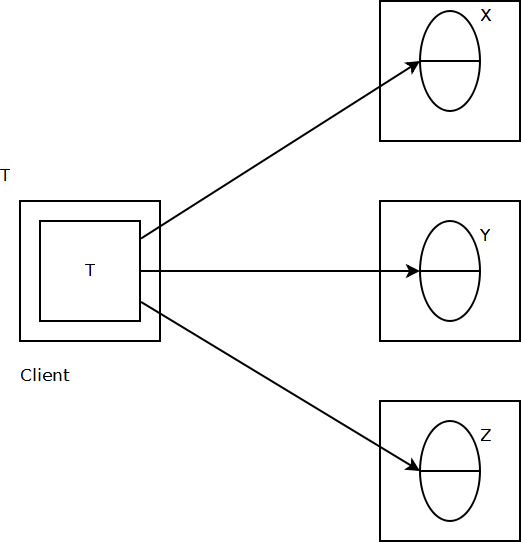
\includegraphics[width=0.4\textwidth]{img/flattransaction}
	\end{center}
	\caption{Flat transaction.}
	\label{fig:flattransaction}
\end{figure}



Nested transactions have finer grained recovery from failures as sub-transactions fail independent. Sub-transactions commit or abort independently, without effect on the outcome of other sub-transactions or enclosing transactions. The effects of sub-transactions becomes durable only when top-level transaction commits [2].

\textbf{Table 2} gives an overview of the operations associated with nested transactions. \textbf{Figure 2} depicts a general model for nested distributed transactions.

\begin{table}
	\caption{Operations in coordinator for nested transactions.}
	\label{tab:api:nestedtransactions}
	\begin{tabular}{p{150px} | p{250px}}
		\textbf{Operation} & \textbf{Description} \\
		\hline
		openSubTransaction (trans) $\rightarrow$ subTrans; 								& \emph{Opens a new subtransaction whose parent in trans and returns a unique subtransaction identifier.} \\
		getStatus (trans) $\rightarrow$ committed, aborted, provisional; 	& \emph{Asks the coordinator to report on the status of the transaction trans. Returns values representing one of the following: committed, aborted or provisional.} \\
		\hline
	\end{tabular}
\end{table}



\begin{figure}
	\begin{center}
		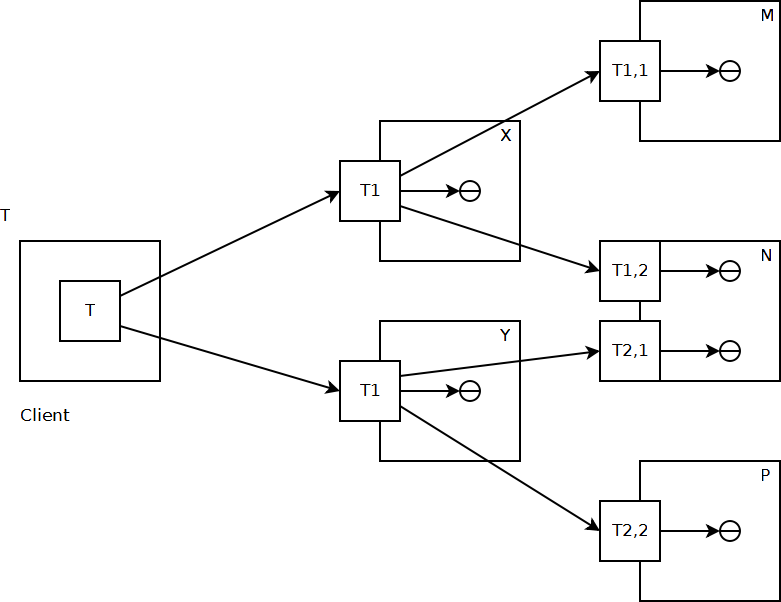
\includegraphics[width=0.6\textwidth]{img/nestedtransaction}
	\end{center}
	\caption{Nested transaction.}
	\label{fig:nestedtransaction}
\end{figure}



\section{Two-phase commit protocols}

The goal of an atomic commit protocol is to ensure that the requirements for transactions are met [1]. The protocol must work correctly, even when some servers fail messages are lost servers are temporarily unable to communicate [2].

The two-phase commit protocol consists out of a votong phase and a completion phase. The completion depends on the outcome of the voting. In the voting phase participants vote for the transaction to be committed or aborted. Once voted for commit, a participant must ensure it can actually carry out the commit. In that case the participant will remain in a \emph{prepared} state. As soon as the coordinator gives a signal that the votes where all in favour of a commit, the result transaction can be committed. In the other case, the transaction is aborted.

The protocol as given in [1] is as follows and is based on the operations listed in \textbf{table 1}; \textbf{figure 3} gives an example scenario of how the protocol is used:

\begin{itemize}
	\item 
		\textbf{Phase 1 (voting phase) :}
		\begin{enumerate}
			\item The coordinator sends a \emph{canCommit?} request to each of the participants in the transaction.
			\item When a participant receives a \emph{canCommit?} request it replies with its vote (\emph{Yes} or \emph{No}) to the coordinator. Before voting \emph{Yes}, it prepares to commit by saving objects in permanent storage. If the vote is \emph{No}, the participant aborts immediately.
		\end{enumerate}
	
	\item 
		\textbf{Phase 2 (completion according to outcome of votes) :}
		\begin{enumerate}
			\setcounter{enumi}{2}
			\item The coordinator collects the votes (including its own).
				\begin{enumerate}[a.]
					\item If there are no failures and all the votes are \emph{Yes}, the coordinator decides to commit the transaction and sends a \emph{doCommit} request to each of the participants.
					\item Otherwise, the coordinator decides to abort the transaction and sends doAbort requests to all participants that voted \emph{Yes}.
				\end{enumerate}
			\item Participants that voted \emph{Yes} are waiting for a \emph{doCommit} or \emph{doAbort} request from the coordinator. When a participant receives one of these messages it acts accordingly and, in the case of commit, makes a \emph{haveCommitted} call as confirmation to the coordinator.
		\end{enumerate}
\end{itemize}


\begin{table}
	\caption{Operations for the two-phase commit protocol.}
	\label{tab:api:twophasecommit}
	\begin{tabular}{p{150px} | p{250px}}
		\textbf{Operation} & \textbf{Description} \\
		\hline
		canCommit (trans) $\rightarrow$ Yes / No; 		& \emph{Call from coordinator to participant to ask whether it can commit a transaction. Participant replies with its vote.} \\
		doCommit (trans); 														& \emph{Call from the coordinator to participant to tell participant to commit its part of a transaction.} \\
		doAbort (trans);															& \emph{Call from coordinator to participant to tell participant to abort its part of the transaction.} \\
		haveCommitted (trans, participant); 					& \emph{Call from participant to coordinator to confirm that it has committed the transaction.} \\
		getDecision (trans) $\rightarrow$ Yes / No; 	& \emph{Call from participant to coordinator to ask for the decision on a transaction when it has voted Yes but still had no reply after some delay. Used to recover from server crash or delayed messages.} \\
		\hline
	\end{tabular}
\end{table}


\begin{figure}
	\begin{center}
		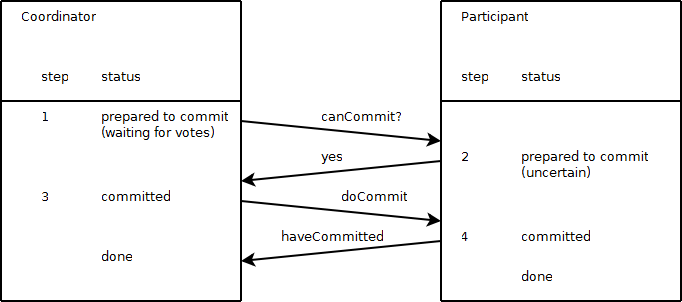
\includegraphics[width=0.6\textwidth]{img/twophasecommit}
	\end{center}
	\caption{Communication in the two-phase commit protocol.}
	\label{fig:twophasecommit}
\end{figure}




For nested transactions, when a subtransaction completes, it either to commits provisionally or aborts. The decision is made indepently. A provisional commit differs from the prepared state in that nothing is backed up in permanent storage. Once all subtransactions have completed, the ones that have been committed provisionally will try to commit their results using the two-phase commit protocol with an additional constraint: if a parent transaction has aborted, the subtransactions will abort as well. A parent transaction however, can commit even if one of its subtransactions has aborted, depending on the implementation [1]. An example of how these transactions are structured is shown in \textbf{figure 4}.

\begin{figure}
	\begin{center}
		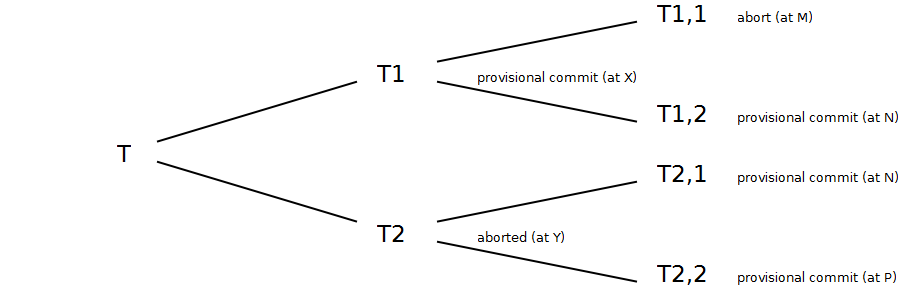
\includegraphics[width=0.8\textwidth]{img/twophasecommitnestedtransaction}
	\end{center}
	\caption{Example scenario for two-phase commit in nested transactions (based on the system depicted in figure 2).}
	\label{fig:twophasecommitnestedtransaction}
\end{figure}


There are two datastructures that are held at the coordinator: a commit list, i.e., a list of all committed (sub)transactions, and an abort list, i.e., a list of all aborted (sub)transactions [2]. The complete datastructure then consists of a list of all transactions, each with a list of their corresponding direct child transactions and commit and abort list [2].



\section{Concurrency}

Servers manage their objects and are responsible for their consistency. Concurrency control is an important aspect of transactions: transactions that access objects in a conflicting way must be handled in the same order by all servers [1].

There are a number of protocols to achieve concurrency control:
\begin{itemize}
	\item \textbf{Locking} : \emph{Locks} are used to facilitate concurrency control. They are held locally at each server. Locks are only released when a transaction has either been committed or aborted at all servers [3].
	\item \textbf{Optimistic concurrency control}
	\item \textbf{Timestamp ordering} : The ordering of transactions can be done through timestamps.
\end{itemize}

\subsection{Locking}

In nested transactions child transactions inherit locks from their parent. When a nested transaction commits, its locks are inherited by its parents, when it aborts, its locks are removed [3].

A transaction is not allowed any new locks after it has released a lock. This results in serial equivalence and requires all of a transaction's accesses to a particular data item to be serialized with respect to accesses by other transactions, and all pairs of conflicting operations of two transactions to be executed in the same order [2]. This results in the \emph{two-phase locking} protocol, consisting of the following two steps:
\begin{enumerate}
	\item \textbf{Growing phase} : New locks can be acquired;
	\item \textbf{Shrinking phase} : No new locks and release of locks.
\end{enumerate}
By releasing locks only at commit or abort, intermediate results can be hidden [2].




\subsection{Optimistic concurrency control}

\subsection{Timestamp ordering}

In the case of distributed transactions, the coordinators must issue globally unique timestamps, which they subsequently correspond to each other. To achieve the same ordering at all severs, the coordinators agree to the ordering of their timestamps [1].




\section{Distributed deadlocks}

To detect deadlocks a wait-for graph can be created. If there exists a cycle in the wait-for graph, a deadlock has occurred. A wait-for graph a directed graph G(\textit{V}, \textit{E}), where the vertices \textit{V} represent transactions and objects, and the edges \textit{E} represent either an object held by a transaction or a transaction waiting for an object [1]. An example is shown in \textbf{figure}. A \emph{distributed deadlock} occurs when there is a cycle in the global \emph{wait-for graph}, as opposed to the local wait-for graph at the server/clients themselves.

A particular problem that occurs in distributed deadlock detection are \emph{phantom deadlocks}. This is a scenario where a deadlock is detected in an outdated wait-for graph. As it may take some time to construct the full graph, a waiting transaction may have already been aborted causing a resource to be no longer required by the corresponding process. Hence, other transactions may be aborted unnecessarily to resolve the phantom deadlock [1]. If transactions are using two-phase locks, they cannot release objects and then obtain more objects, and phantom deadlock cycles cannot occur in the way suggested here [1].

There exist centralized and decentralized approaches to construct a global wait-for graph. In the following paragraphs we will discuss an example of both.


\subsection{Centralized deadlock detection}

In centralized deadlock detection one server has the responsibility for detecting deadlocks. Each time after a certain time interval, each server sends the lastest copy of its local wait-for graph to this global deadlock detector. When a deadlock is detected, it makes a decision on how to resolve it and notifies the servers which transactions to abort [1].

This kind of deadlock detection has some obvious disadvantages [1]:
\begin{itemize}
	\item Poor availability;
	\item Lack of fault tolerance;
	\item Poor scalability.
\end{itemize}


\subsection{Distributed deadlock detection: the edge-chasing algorithm}

A distributed approach to deadlock detection uses a technique called \emph{edge chasing} or \emph{path pushing}. Here, the global wait-for graph is not constructed, but each of the servers involved has knowledge about some of its edges. The servers attempt to find cycles by forwarding messages called \emph{probes}, which follow the edges of the graph throughout the distributed system. A probe message consists of transaction wait-for relationships representing a path in the global wait-for graph [1].

Edge-chasing algorithms have three steps [1]:
\begin{enumerate}
	\item \textbf{Initiation} : When a server notes that a transaction T starts waiting for another transaction U, where U is waiting to access an object at another server, it initiates detection by sending a probe containing the edge < T $\rightarrow$ U > to the server of the object at which transaction U is blocked. If U is sharing a lock, probes are sent to all the holders of the lock. Sometimes further transactions may start sharing the lock later on, in which case probes can be sent to them too.
	\item \textbf{Detection} : Detection consists of receiving probes and deciding whether a deadlock has occurred and whether to forward the probes. The global wait-for graph is built one edge at the time. As soon as cycle is detected, a deadlock has occurred.
	\item \textbf{Resolution} : When a cycle is detected, a transaction in the cycle is aborted to break the deadlock.
\end{enumerate}


\section*{References}

\begin{enumerate}[1]
	\item G. Coulouris, J. Dollimore, T. Kindberg and G. Blair, "Distributed Systems: Concepts and Design (5th Edition)", M. Horton, Red., Addison-Wesley, 2011, p. 1063.
	\item W. Joosen, 2013, "Distributed Systems - Transactions - I", IBBT-DistriNet, KULeuven
	\item W. Joosen, 2013, "Distributed Systems : Transactions - Part 2", IBBT-DistriNet, KULeuven
\end{enumerate}